\section{Introducción}

El presente documento recoge el diseño, la implementación y la validación de
una red empresarial multi-sede que da respuesta a los requerimientos planteados
en el proyecto final de Comunicaciones II como se muestra en la siguiente imagen:

\begin{figure}[H]
      \centering
      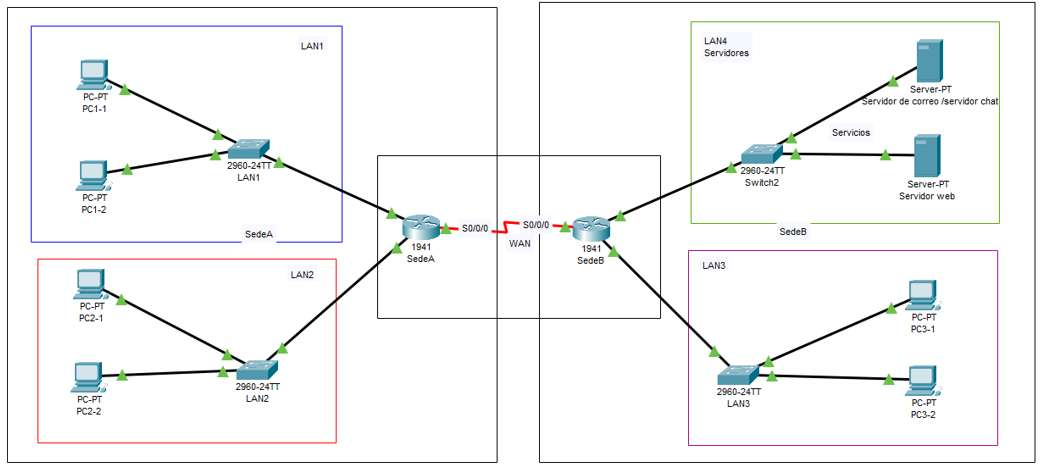
\includegraphics[width=1\textwidth]{images/base.jpg}
      \caption{Diagrama de la red multi-sede a implementar.}
\end{figure}

La red integra tres segmentos LAN con
un total de 1.650 usuarios finales, distribuidos en áreas con capacidades de 850,
600 y 200 hosts respectivamente, y debe garantizar conectividad plena entre todas
las sedes mediante enrutamiento dinámico.

Un requisito del proyecto es la operación en doble stack, de modo que
cada dispositivo de la topología cuente con direccionamiento tanto IPv4 como IPv6.
El espacio de direcciones IPv4 asignado al Grupo 1 es \texttt{172.16.192.0/19},
y el prefijo IPv6 de referencia es \texttt{2001:dbe:bef9::/48}. El diseño del
direccionamiento parte de estos bloques y aplica un factor de crecimiento del 10\%
sobre la cantidad de usuarios de cada área, con el fin de garantizar escalabilidad
sin necesidad de renumerar la red en el corto plazo.

Adicionalmente, la red debe soportar tres servicios de aplicación accesibles desde
todos los segmentos: un servicio web, un servicio de correo electrónico y un
servicio de mensajería instantánea. Este último corresponde a una implementación
propia desarrollada en C sobre sockets TCP, con soporte para múltiples usuarios
simultáneos, salas de chat y visualización de usuarios conectados, operando sobre
terminal tanto en el servidor Linux como en los clientes Windows que se puede ver en el siguiente repositorio: \url{https://github.com/Juanes7222/Socket.git}.

El documento se organiza siguiendo la estructura requerida por el enunciado del
proyecto: inicia con la descripción de requerimientos, continúa con las decisiones
de diseño y la configuración de los equipos, y cierra con el diseño y ejecución de
pruebas de validación, los problemas encontrados durante la implementación y las
conclusiones del proceso.